\chapter{实验设计与讨论}
本章对前面提到的所有模型都设计了相应的实验,同时做了多组对照试验,以验证我们对模型改进的可行性和有效性。

\section{实验数据集与预处理}
\subsection{实验数据集}
实验开始前调研了与本文任务类似的数据集,调研结果发现高质量的可用于跨界服务平台的中文语料数据集相对匮乏,例如对话类数据集部分输入为语音而不是
文本,再如科大讯飞阿里小蜜有着海量有商业价值数据的公司没有公开数据集。为此,我们选择在已有数据集上做标注补充和扩展,构建了跨界服务相关的中文
预料数据集。

\begin{figure}[htbp]
    \centering
    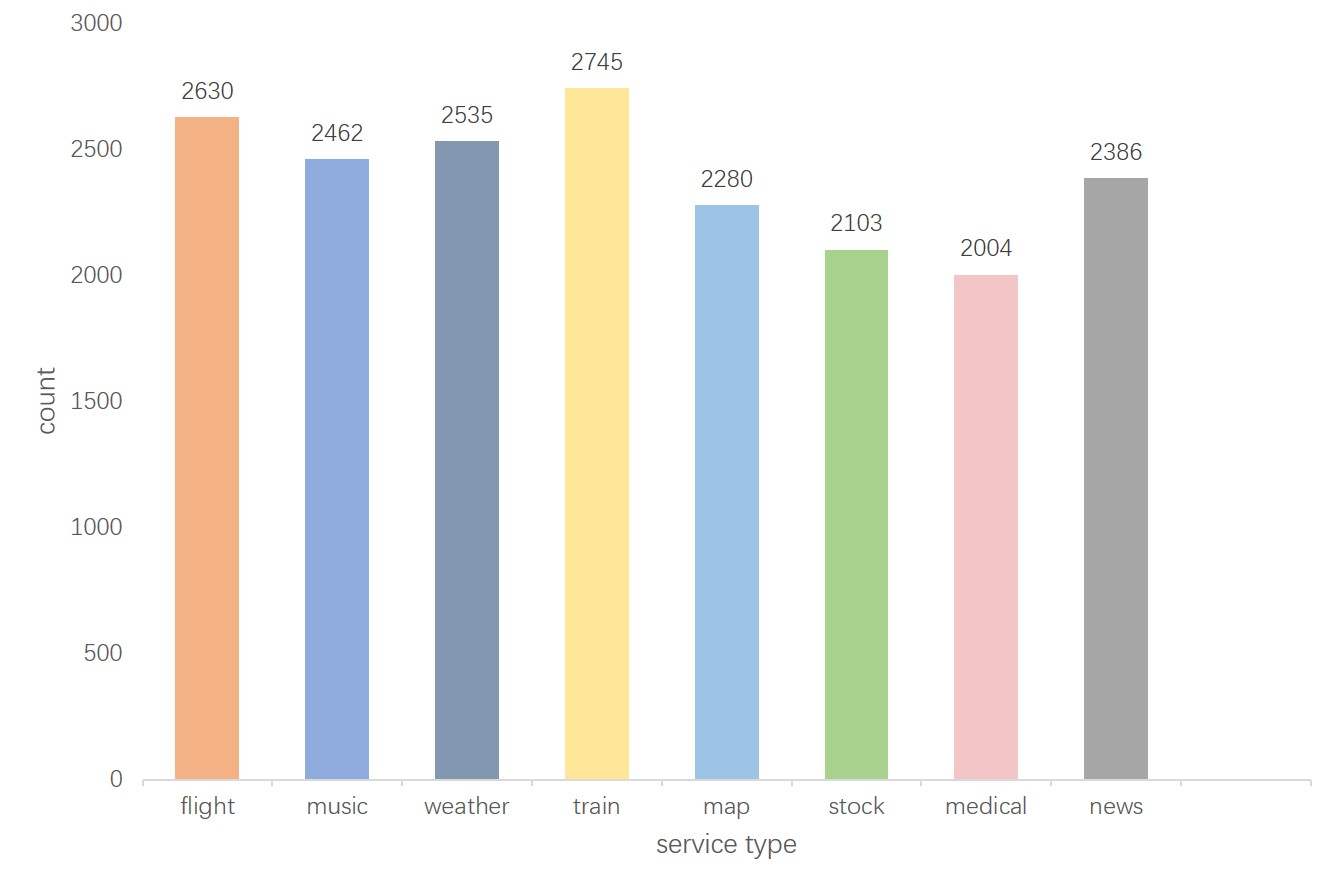
\includegraphics[width=15cm]{./images/count.jpg}
    \caption{数据集分布图}
    \label{fig:count}
  \end{figure}

SMP2019中文人机对话技术评测自然语言理解任务中提供了SMP2019ECDT数据集,其中主要包括垂直类,闲聊类和知识问答,我们结合跨界服务平台系统内部常用
服务,从垂直类中选择部分数据做标注扩充以及数据扩充。本文筛选了合跨界服务平台中用户使用较多的几类服务的语料信息,包括“航班flight”,“音乐music”,
“天气weather”,“火车train”,“地图map”,“股票stock”,“医疗medical”,“新闻news”共八大类服务,再根据这些服务的接口构建接口类别的全集,例如“query”,“play”,“order”等;同时确定了服务接口以后,服务接口调用
时的参数(语义槽)也就确定了,例如“songName”,“singer”,“startCity”,“endCity”等,可见接口和服务参数都是和服务强相关的。例如,当服务类型被判定为
“天气weather”时,接口类型为“query”,参数(语义槽)为“city”。

SMP2019ECDT数据集中与跨界服务平台系统内八大服务相关的数据量并不大,因此本文对原有数据集做了扩充。扩充工作主要分为两部分:横向扩充和纵向扩充,横向
扩充的直觉来源于同一个语义的句子不同人的表述会不同,例如“杭州具体天气怎么样?”和“杭州今天多少度?”,因此考虑对同种语义的句子做横向扩充,这里我们借助
了百度和必应(微软bing)两大搜索引擎的搜索联想补全功能。横向扩充完的句子标签中的服务类别和接口类别不用变,只需要修改语义槽标注。
如图\ref{fig:baidu},\ref{fig:bing}所示,想要扩展火车服务的查询接口的语料数据,再搜索引擎输入“成都到杭州火车”,利用搜索引擎的联想补全功能
达到扩充的目的。

\begin{figure}[htbp]
    \centering
    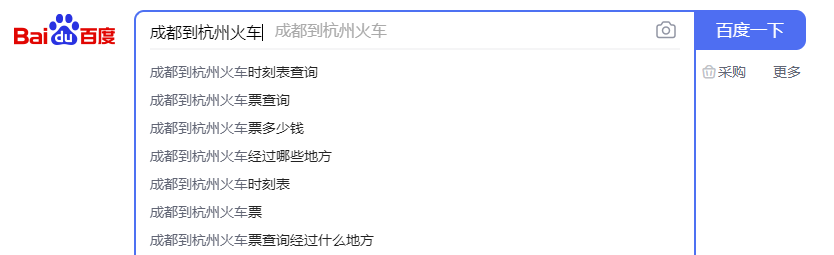
\includegraphics[width=15cm]{./images/baidu.png}
    \caption{数据横向扩充图1}
    \label{fig:baidu}
  \end{figure}

  \begin{figure}[htbp]
    \centering
    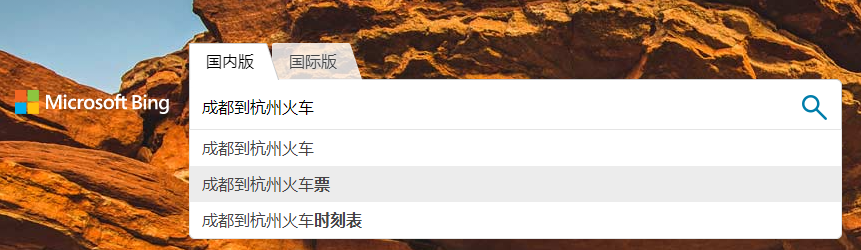
\includegraphics[width=15cm]{./images/bing.png}
    \caption{数据横向扩充图2}
    \label{fig:bing}
  \end{figure}

数据集纵向扩充是组织跨界服务课题组和实验室同学填写问卷,让被调研者输入相应服务的查询语句,收集起来对语句进行人工标注,完成数据集的扩容。
每个人对同一语义的表达会有差异,有差异的数据对训练出泛化能力好的数据是大有裨益的。最终经过课题组同学的努力,共构建了19145条数据组成实验
数据集,每条数据都包含服务类别标签、接口类别标签和参数(语义槽)标签。



\subsection{预处理}

\section{评价指标}
评价指标用于评估模型的性能,对于服务分类任务,本文采用准确率(Accuracy)来评估模型;对于接口分类
任务,同样采用准确率(Accuracy)来评估模型;对于参数(语义槽)填充任务,采用$F_1$值来评估模型。同时引入
句子准确率(Sentence Accuracy)作为更严格的指标来评估模型,即一个句子只有在三项任务同时正确时才会被计入
句子准确率中。

以服务类别标签的混淆矩阵\ref{fig:bing}为例介绍以上指标的计算方法

% \begin{table}[htb]
%   \centering
%   \caption{服务类型混淆矩阵}
%   \label{tab:RelatedResearchInChina}
%     \begin{tabular}{p{2cm}|p{4cm}}
%       \toprule
%       % & \multicolumn{1}{m{60mm}}{\heiti\centering 相关研究成果}
%       \multicolumn{1}{l|}{\heiti } & \multicolumn{1}{l|}{\heiti 相关研究内容} \\
%       \midrule
      
%       \bottomrule
%     \end{tabular}
% \end{table}


\begin{tabular}{|c|c|c|c|c|}
  \hline
  \multirow{2}{*}{Multi-Row}&
  \multicolumn{2}{c|}{Multi-Column}&
  \multicolumn{2}{c|}{\multirow{2}{*}{Multi-RowandCol}} \\
  \cline{2-3}
    & column-1&column-2 & \multicolumn{2}{c|}{}\\
  \hline
  label-1 & label-2&label-3 & label-4& label-5\\
  \hline
  \end{tabular}

  \begin{tabular}{|c|c|c|c|}
    \hline
    \multicolumn{2}{c|}{\multirow{2}{*}{两行两列}}&
    \multicolumn{2}{c|}{预测值}\\
    \cline{3-4}
     & &flight & music \\
     \hline
    label-1 & label-2&label-3 & label-4\\
    \hline
    \end{tabular}


    

    % \begin{table}[htb]
    %   \centering
    %   \caption{服务类型混淆矩阵}
    %   \label{tab:hunxiao}
    %   \begin{tabular}{|l|l|l|l|l|l|l||l|l|l|}
    %     \hline
    %     \multicolumn{2}{c|}{\multirow{2}{*}{两行两列}}&
    %     \multicolumn{8}{c|}{预测值}\\
    %     \cline{3-10}
    %      &flight & music & weather & train & map &stock &medical & news \\
    %     \hline
    %     \end{tabular}
    % \end{table}

\section{实验设置}

\section{实验结果与分析}